\section{Definition}

\vspace{\parskip}

\begin{definition}[Graphs] \index{graphs} \index{vertices} \index{edges}
    A graph is defined as a tuple $G=(V,E)$ where $V$is an arbitrary non-empty finite set, whose elements are called vertices or nodes; and $E$ is a set of pairs of elements of $V$, which we call edges. For an undirected graph, the edges are unordered pairs ${u,v}$. In a directed graph, the edges are ordered pairs $(u,v)$.
\end{definition}

\begin{definition}[Neighbors and Degrees] \index{neighbors} \index{predecessor} \index{successor} \index{degree} \index{in-degree} \index{out-degree}
    For any edge $uv$ in an undirected graph, we call $u$ neighbor of $v$ and vice versa, and we say that $u$ and $v$ are adjacent. The degree of a node is its number of neighbors.

    In directed graphs, for every edge $u \to v$, we call $u$ a predecessor of $v$, and we call $v$ a successor of $u$. The in-degree of a vertex is its number of predecessors; the out-degree is its number of sucessors.
\end{definition}

\begin{definition}[Subgraphs] \index{subgraphs}
    A graph $G' = (V',E')$ is a subgraph of $G=(V,E)$ if $V' \subseteq V$ and $E' \subseteq E$. A proper subgraph of $G$ is any subgraph that is not $G$ itself.
\end{definition}

\section{Representations of Graphs}

\subsection{Adjacency List}

\vspace{\parskip}

\begin{definition}[Adjacency List] \index{adjacency-list}
    The adjacency-list representation of a graph $G=(V,E)$ consists of an arrray \textit{Adj} of $|V|$ lists, one for each vertex in $V$. For each $u \in V$, the adjacency list \textit{Adj[u]} contains all the vertices $v$ such that there is an edge $(u,v) \in E$. That is, \textit{Adj}[u] contains all the vertices adjacent to $u$ in $G$.
\end{definition}

\begin{figure}[htbp]
    \centering
    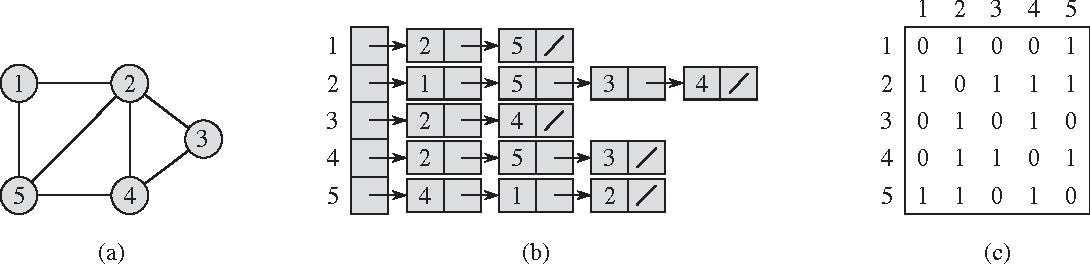
\includegraphics[width=\linewidth]{figures/undirected_graph.pdf}
    \caption{Representations of undirected graph: (a) the graph; (b) adjacency list of the graph; (c) adjacency matrix of the graph.}
    \label{<label>}
\end{figure}

\section{Breadth-first Search} \index{breadth-first search (BFS)}

Given a graph $G=(V,E)$ and a distinguished source vertex $s$, breadth-first search systematically explores the edges of $G$ to discover every vertex that is reachable from $s$. Breadth-first search expands the frontier between disvoered and undiscovered vertices uniformly across the breadth of the frontier. The algorithm discovers all vertices at distance $k$ from $s$ before discovering any vertices at distance $k+1$.

